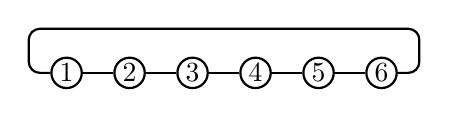
\begin{tikzpicture}[thick, scale=0.8]
	\def\numNodes{6}
	\pgfmathtruncatemacro{\numNodess}{\numNodes-1}
	
	% Nodes
	\foreach \x in {1,...,\numNodes}{
		\node (node \x) at (\x,0)
		      [draw, circle, inner sep=0.1em]
		      {\x};
	}
	
	% Wires between nodes
	\foreach \x in {1,...,\numNodess}{
		\pgfmathtruncatemacro{\xx}{\x+1}
		\draw (node \x) -- (node \xx);
	}
	
	% Wrap-around wire
	\draw [rounded corners]
	      (node \numNodes)
	   -| ++(0.6,0.7)
	   -| ([shift={(-0.6,0)}] node 1.center)
	   -- (node 1)
	    ;
\end{tikzpicture}

